\documentclass[../../main]{subfiles}
\graphicspath{{\subfix{../../Images/}}}

\begin{document}

W tej części pracy będzie przedstawiona dekompozycja oprogramowania systemowego przedstawionego w poprzedniej części w architekturach z systemem operacyjnym i wirtualizacją, a dokładnie: systemu operacyjnego i hiperwizora. Następnie oprogramowanie odpowiadające za zarządzanie dostępem do zasobów jednostki obliczeniowej będzie wyodrębnione ze wspomnianego przed tym oprogramowania systemowego dla przeprowadzenia analizy w następnej części pracy.

Należy zauważyć, że celem tej pracy nie jest omówienie wszystkich elementów oprogramowania systemowego. Pozostałe elementy oprogramowania systemowego będą wspomniane, jeżeli będzie na to potrzeba, tylko w sposób ogólny, pozwalający na prześledzenie udziału oprogramowania zarządzającego zasobami jednostką obliczeniową w ogólnej architekturze oprogramowania systemowego, oraz umożliwiający wyodrębnienie tej części dla dalszej analizy. % TODO: check first centense punktuation and structure.

\subsection{Dekompozycja}
\begin{figure}[h]
    \centering
    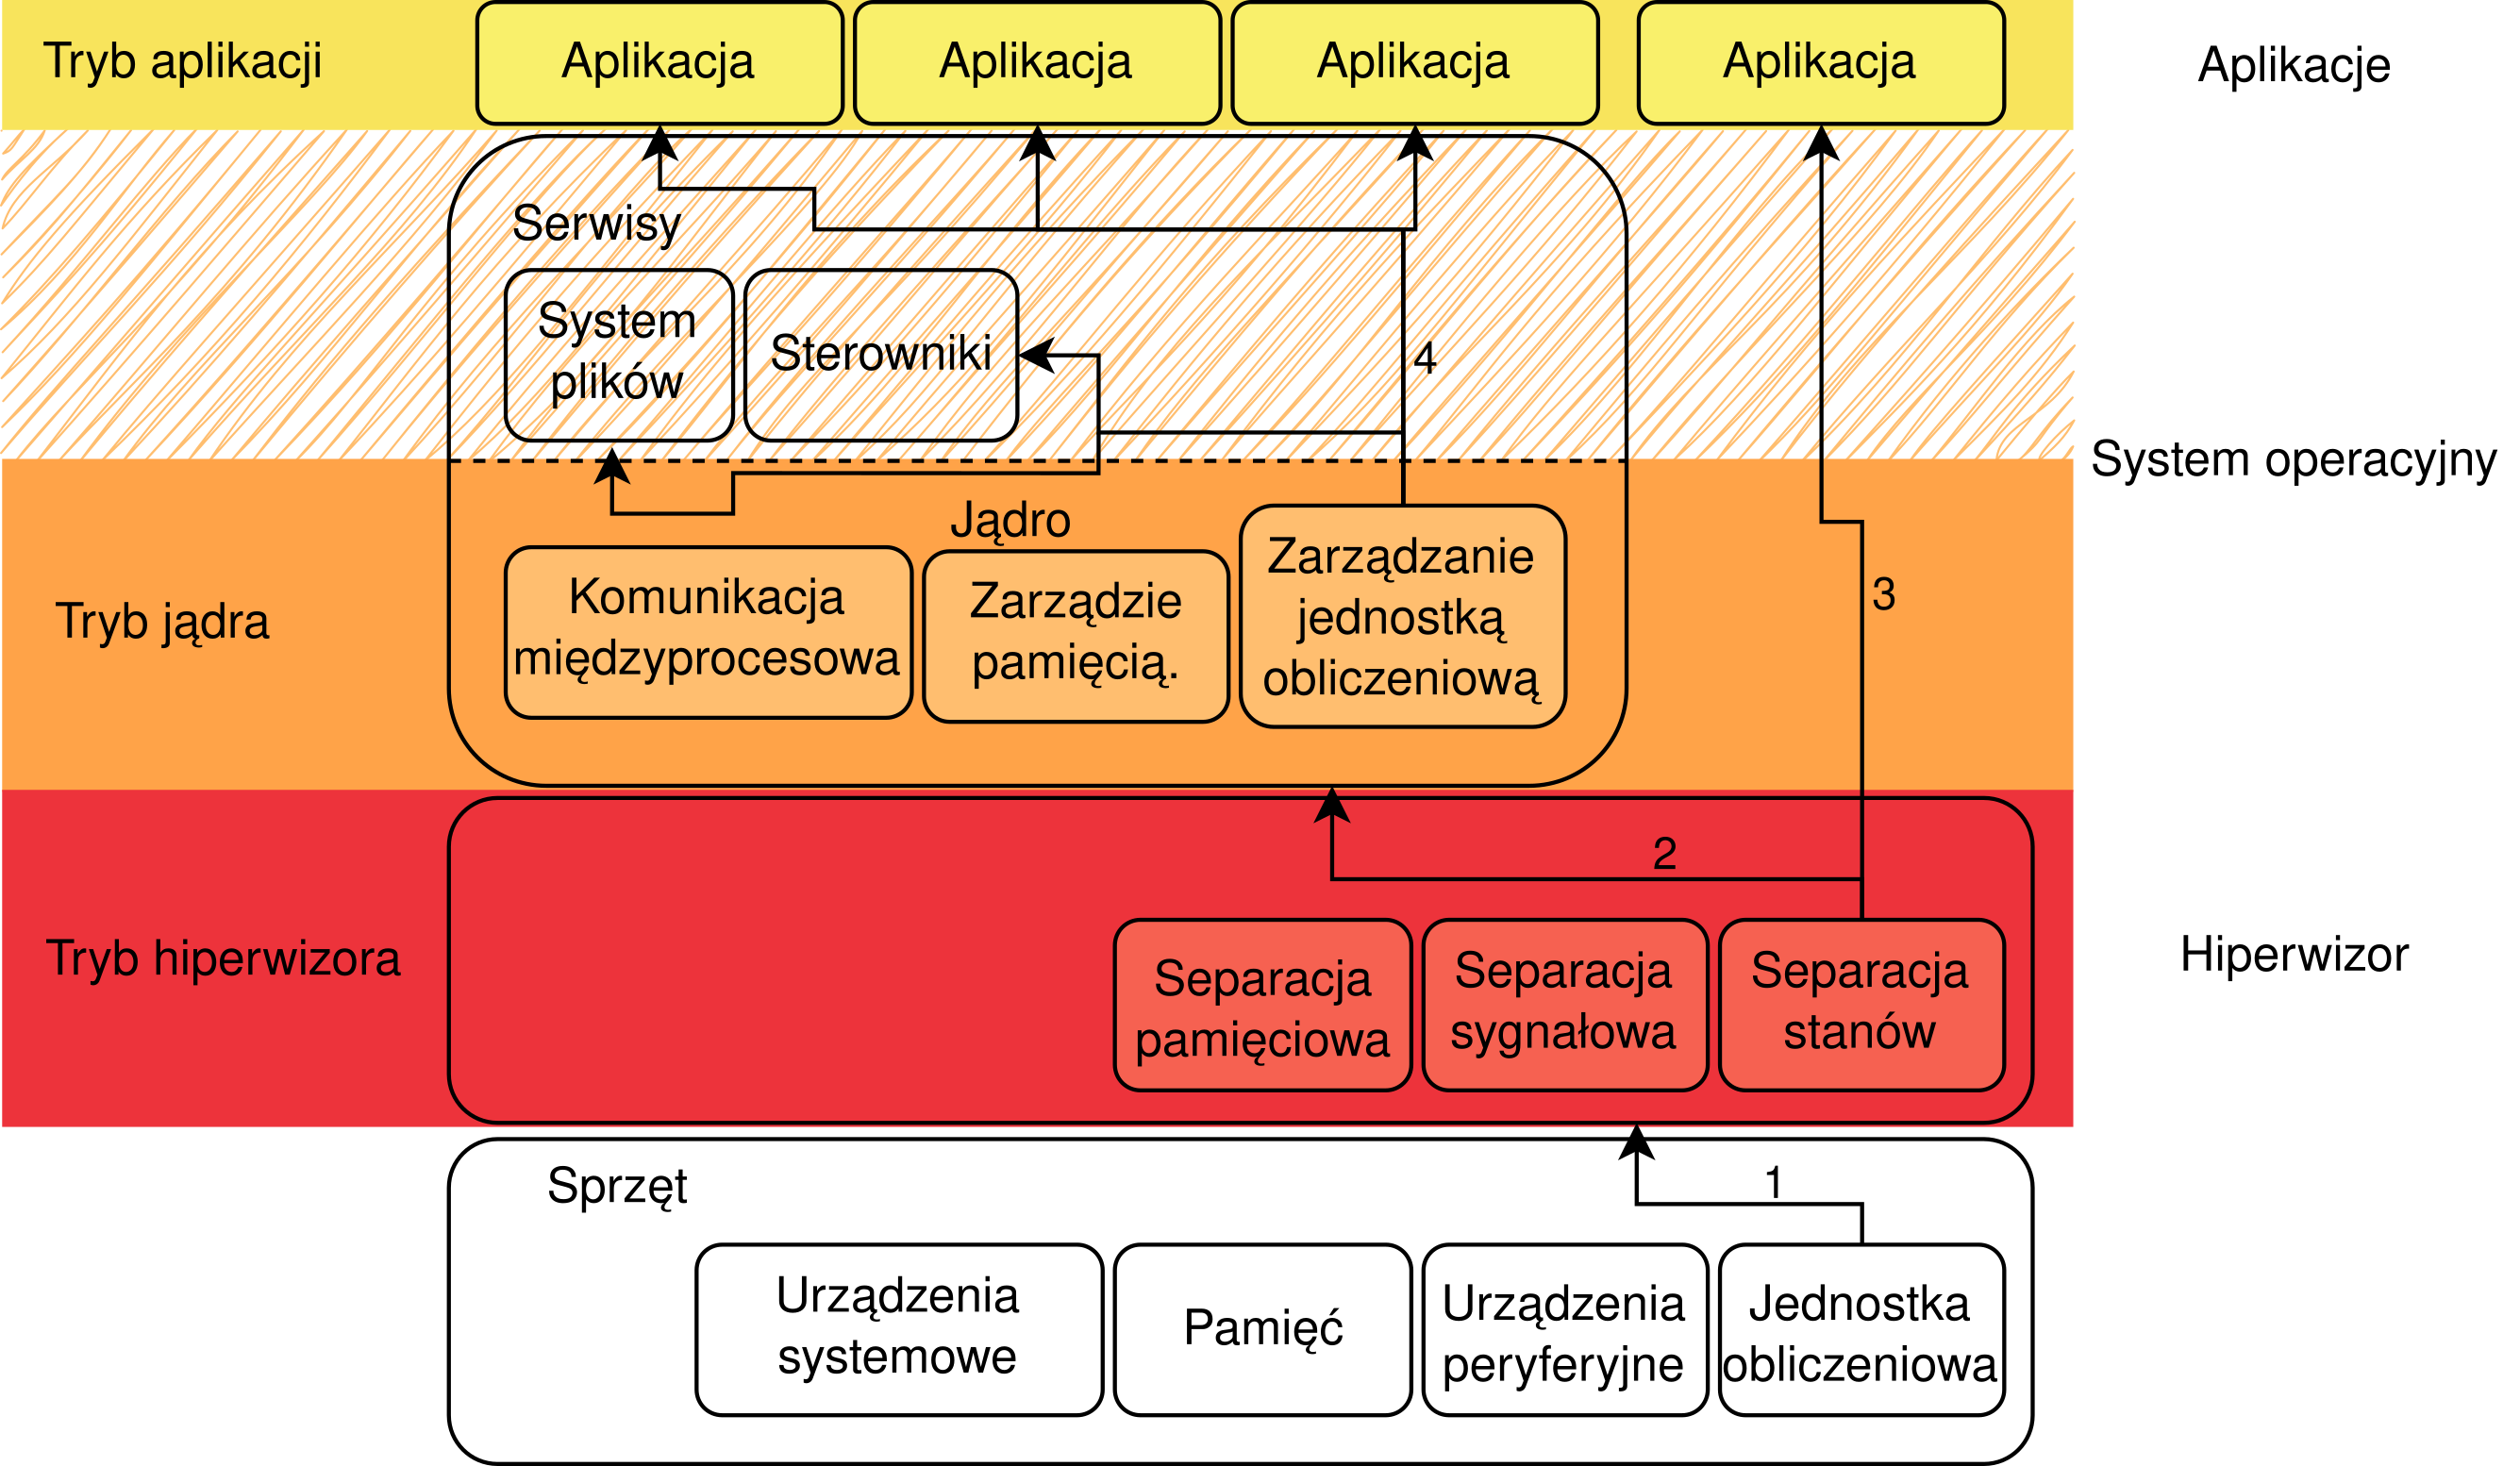
\includegraphics[width=\textwidth]{Images/cpu-resources-multiplexing.png}
    \caption{Przydzielenie dostępu do zasobów jednostki obliczeniowej przez oprogramowanie systemowe: system operacyjny i hiperwizor}
    \label{fig:cpu-resources-mult}
\end{figure}

Jak wspomniano poprzednio, z punktu widzenia zarządzania zasobami jednostki obliczeniowej są ciekawe dwa rodzaje oprogramowania systemowego: system operacyjny i hiperwizor. Na \cref{fig:cpu-resources-mult} jest pokazane przydzielenie zasobów jednostki obliczeniowej przy użyciu tego oprogramowania systemowego, kolorami są odznaczone tryby, w których znajduje się jednostka obliczeniowa podczas wykonywania instrukcji pewnego oprogramowania, zacieniony obszar wskazuje, że serwisy systemu operacyjnego mogą być wykonywane zarówno w trybie jądra jak i w trybie aplikacji (zależy od architektury systemu operacyjnego: mikrokernel lub monolityczny kernel). Strzałkami jest odznaczone przydzielenie zasobów jednostki obliczeniowej do pewnego oprogramowania przez pewną logikę w oprogramowaniu systemowym. Ten rysunek demonstruje architekturę z wirtualizacją, zaś architektura bez wirtualizacji wykorzystująca tylko system operacyjny może być pokazana usuwając z \cref{fig:cpu-resources-mult} cały hiperwizor i strzałkę o numerze 3. W takim przypadku strzałka o numerze 1 będzie wskazywała wprost na system operacyjny.

Jest to struktura hierarchiczna, tzn. (numery punktów są odpowiednie do numerów strzałek na \cref{fig:cpu-resources-mult}):

\begin{enumerate}
    \item Hiperwizor otrzymuję kontrolę nad wszystkimi zasobami jednostki obliczeniowej i przydziela je do oprogramowania, które on uruchamia: system operacyjny (strzałka nr 2 na \cref{fig:cpu-resources-mult}) lub aplikacja (strzałka nr 3 na \cref{fig:cpu-resources-mult}), spędzając na ten proces pewną część otrzymanych zasobów;
    \item System operacyjny otrzymuję od hiperwizora pewną część zasobów jednostki obliczeniowej (strzałka nr 2 na \cref{fig:cpu-resources-mult}) i rozprowadza je do serwisów lub aplikacji (strzałki o wspólnym numerze 4 na \cref{fig:cpu-resources-mult}), spędzając na ten proces pewną część otrzymanych zasobów;
    \item Aplikacja, która jest uruchomiona bez systemu operacyjnego otrzymuje przydzielone zasoby od hiperwizora (strzałka nr 3 na \cref{fig:cpu-resources-mult}) i zaczyna wykonywać swoją pracę;
    \item Aplikację i serwisy, uruchomione przez system operacyjny, otrzymują przydzielone im zasoby przez system operacyjny (strzałki o wspólnym numerze 4 na \cref{fig:cpu-resources-mult}) i zaczynają wykonywać swoją pracę.
\end{enumerate}

W systemie operacyjnym funkcjonalność przydzielenia zasobów jednostki obliczeniowej jest jedna z trzech kluczowych (pozostałe dwie: komunikacja międzyprocesowa i zarządzanie pamięcią). Natomiast w hiperwizorze jest to jedna ze sposobów separacji (pozostałe dwie: separacja sygnałowa i separacja pamięciowa; \hyperref[sec:zalacznik-3]{załącznik nr 3}).

Logikę lub kod, który odpowiada za zarządzanie zasobami jednostki obliczeniowej zarówno w systemie operacyjnym jak i hiperwizorze (pomiędzy strzałkami 1 i 2, oraz pomiędzy strzałkami 2 i 4, \cref{fig:armv8-m-context-switch}) można nazwać nadzorcą (ang. supervisor). Takie nazewnictwo będzie stosowane w dalszej części pracy. Nadzorcę można także podzielić na dwie części: dyspozytora (ang. dispatcher) i planistę (ang. scheduler).

Centrum uwagi tej pracy jest planista.

\subsection{Wyodrębnienie}
\begin{figure}[H]
    \centering
    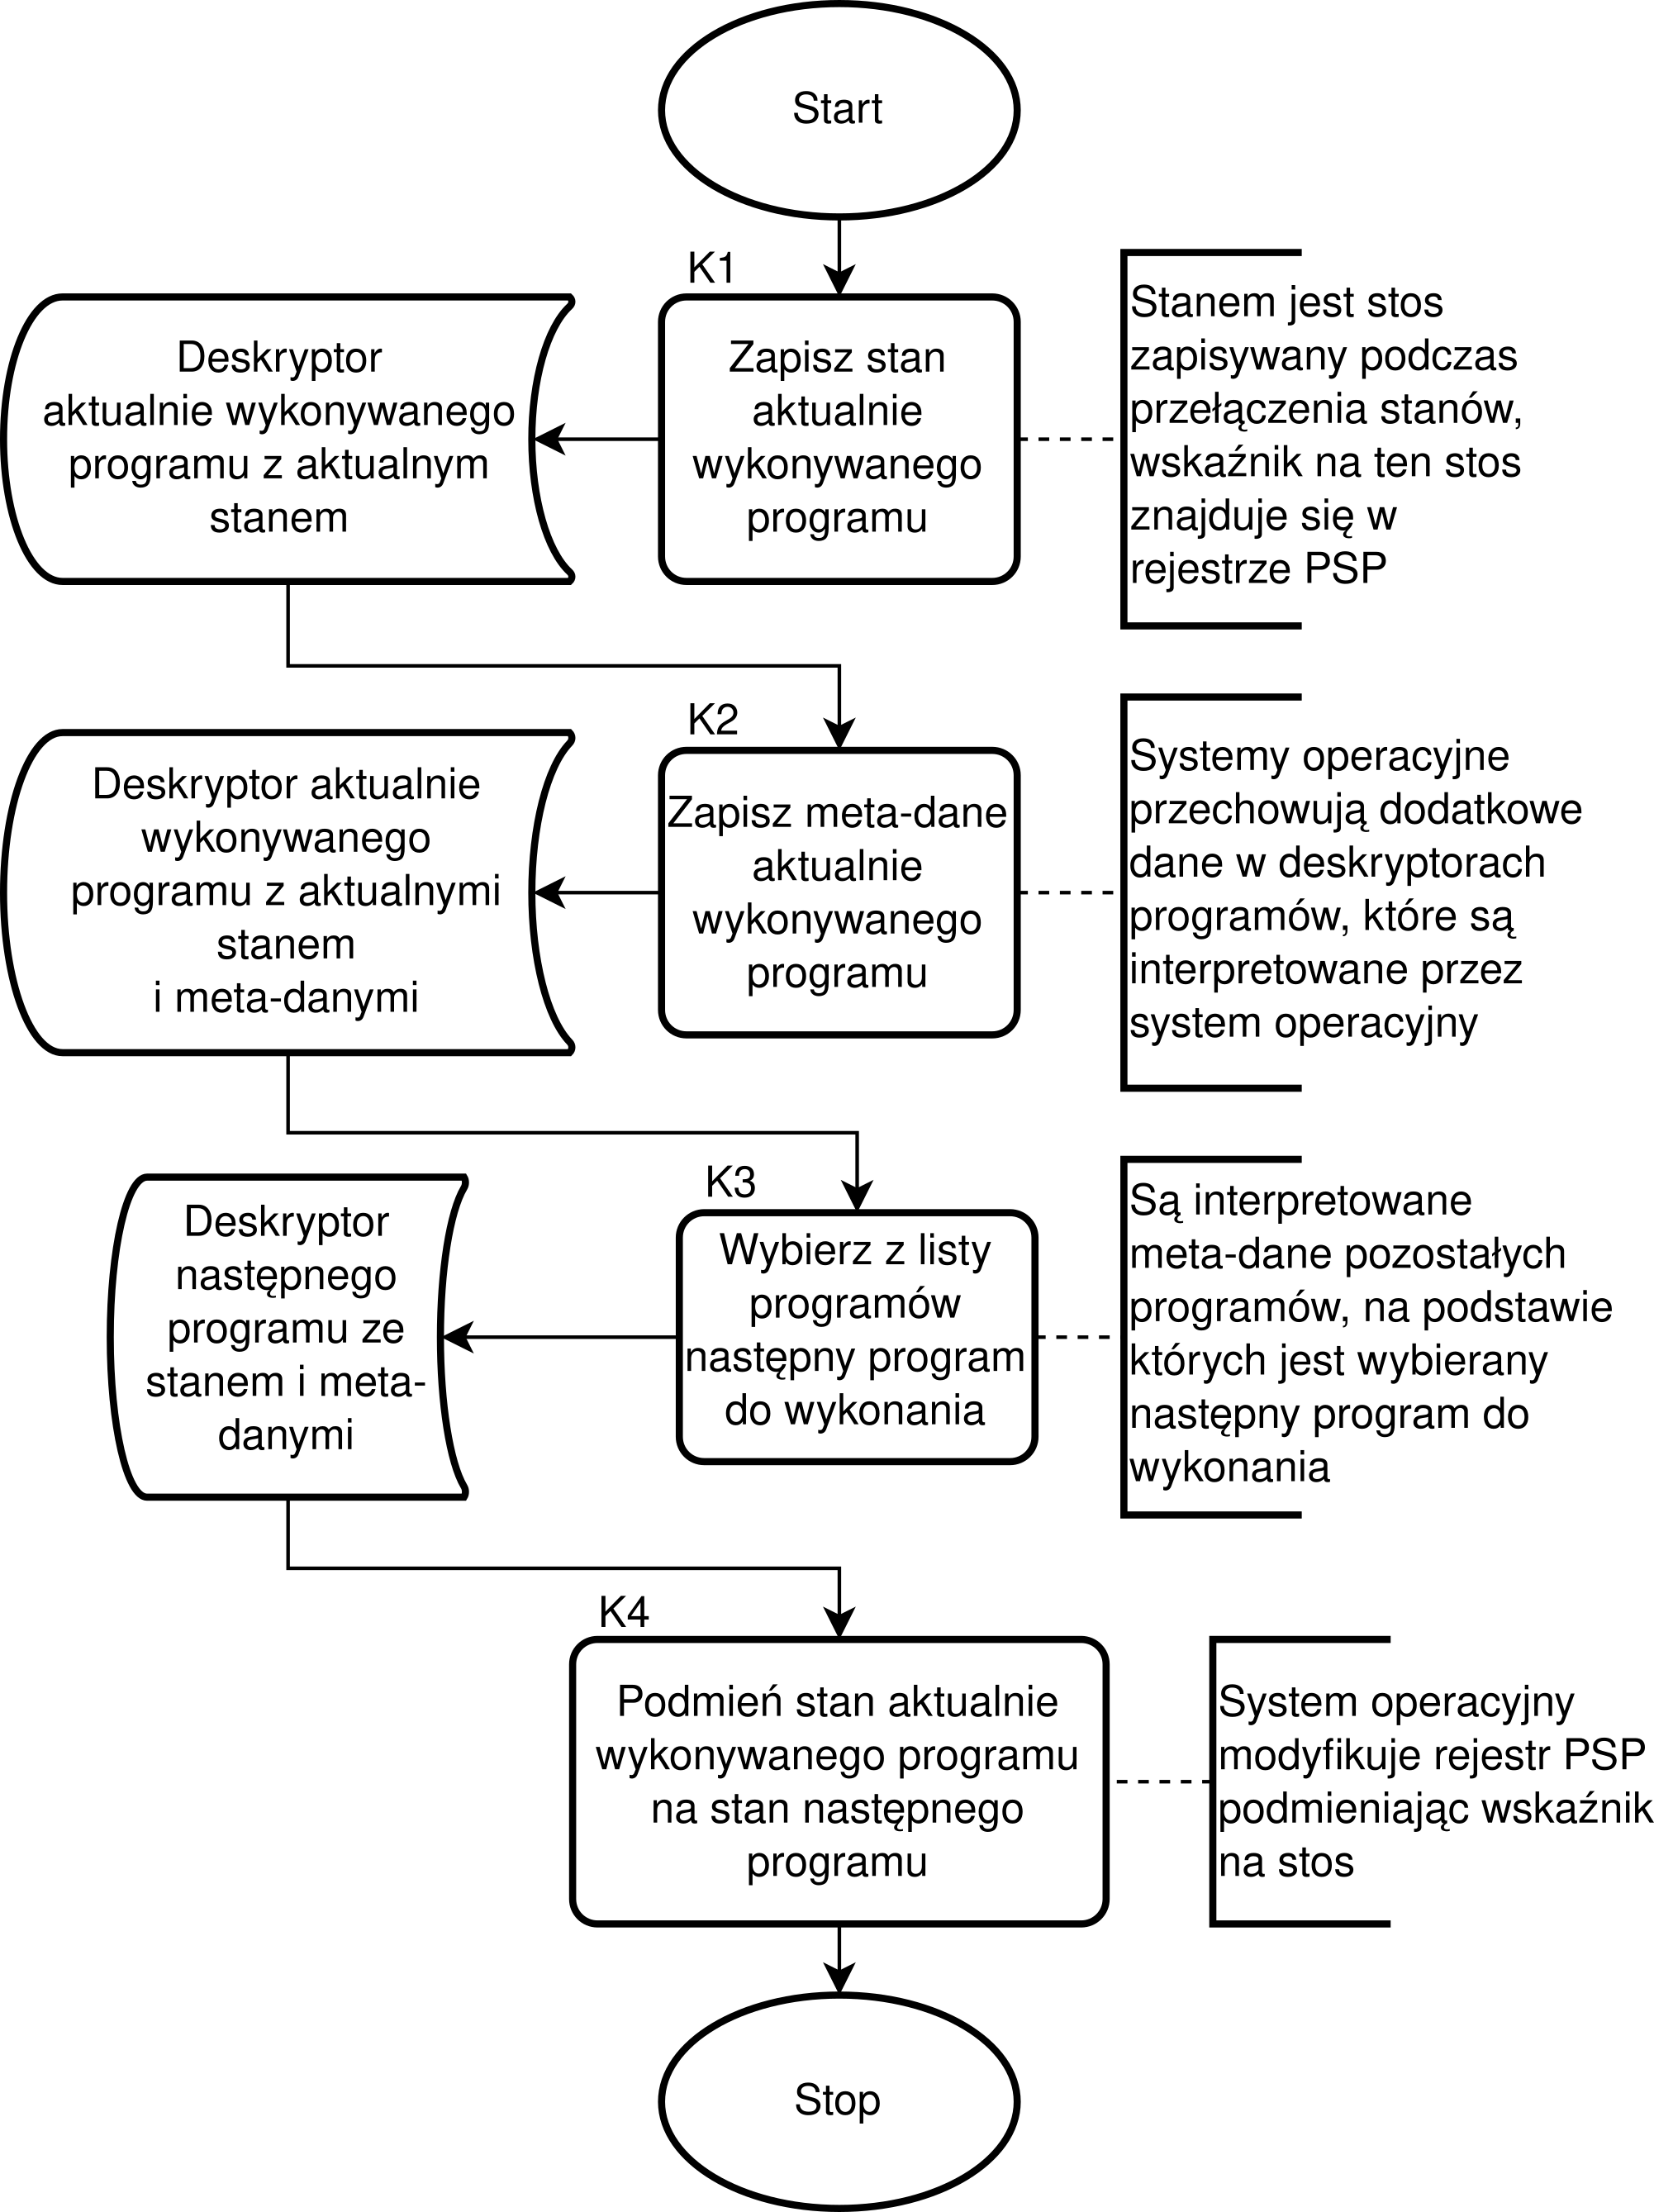
\includegraphics[width=0.85\textwidth]{Images/context-switching-armv8-m.png}
    \caption{Ogólna logika przełączenia kontekstu}
    \label{fig:armv8-m-context-switch}
\end{figure}

Wspomniany w poprzedniej części nadzorca jest wyłowy łany tylko w pewnych, szczególnie zdefiniowanych przypadkach, aby wykonać przełączenie kontekstu. Wywoływany on może być periodycznie, za pomocą periodycznego przerwania, lub "na żądanie" za pomocą przerwania systemowego (w przypadku \acrshort{arm}'u jest to przerwanie generowane instrukcjami \acrshort{svc} i \acrshort{hvc}).

Po wywołaniu nadzorcy następuje przełączenie kontekstu. Na \cref{fig:armv8-m-context-switch} są ogólnie opisane kroki przełączania kontekstu. Przy czym kroki K1, K2 i K4 (\cref{fig:armv8-m-context-switch}) są wykonywane przez dyspozytora, i tylko krok K3 (\cref{fig:armv8-m-context-switch}) jest wykonywany przez planistę.

Zadaniem dyspozytora jest otrzymywanie informacji i przekierowanie jej w odpowiednim formacie do planisty (kroki K1 i K2 na \cref{fig:armv8-m-context-switch}), który podejmuje decyzję na podstawie zdefiniowanych reguł (krok K3 na \cref{fig:armv8-m-context-switch}), i informuje o tym dyspozytora. Dyspozytor podejmuje odpowiednie dla podjętej decyzji działania (krok K4 na \cref{fig:armv8-m-context-switch}).

Więc wejściem do planisty jest lista deskryptorów procesów oczekujących na przydzielenie zasobów obliczeniowych oraz ilość dostępnych zasobów obliczeniowych. Wyjściem jest deskryptor procesu z przydzielonymi zasobami jednostki obliczeniowej. Planista podejmuję decyzję na podstawie wstępnie zdefiniowanych reguł.

\end{document}